\documentclass[preprint,12pt,authoryear]{elsarticle}
\usepackage{amsmath,amssymb}
\usepackage{booktabs}
\usepackage{graphicx}
\usepackage{siunitx}
\usepackage{hyperref}
\usepackage{longtable}
\usepackage[margin=1in]{geometry}
% Generated by rfsrealloc.pipeline; do not edit.

\newcommand{\valabsorbableDrawdown}{2.0}
\newcommand{\valadditionalAB}{250}
\newcommand{\valadditionalBBD}{180}
\newcommand{\valadditionalExactRF}{766.8}
\newcommand{\valadditionalRF}{770}
\newcommand{\valadditionalRFReportedBasis}{760}
\newcommand{\valbankBaseline}{4.37}
\newcommand{\valbankOutFirstAllTwoZeroTwoSeven}{3.37}
\newcommand{\valbankOutFirstEqual}{3.01}
\newcommand{\valbankOutFirstSetTwo}{3.37}
\newcommand{\valbankOutSecondAllTwoZeroTwoSeven}{1.56}
\newcommand{\valbankOutSecondEqual}{1.57}
\newcommand{\valbankOutSecondSetTwo}{2.33}
\newcommand{\valbankRia}{3.6}
\newcommand{\valbtFirstTargetYear}{2021}
\newcommand{\valbtLastTargetYear}{2027}
\newcommand{\valbtMaeAllSecond}{1,003}
\newcommand{\valbtMaeEqual}{969}
\newcommand{\valbtNTargetYears}{7}
\newcommand{\valbtNYearsFullyUnknownEqual}{6}
\newcommand{\valbtUnknownAllSecondFirst}{160}
\newcommand{\valbtUnknownAllSecondSecond}{1,760}
\newcommand{\valbtUnknownEqualFirst}{960}
\newcommand{\valbtUnknownEqualSecond}{880}
\newcommand{\valbtUnknownShareAllFirst}{1.0}
\newcommand{\valbtUnknownShareAllSecond}{0.876}
\newcommand{\valbtUnknownShareAllSecondFirst}{0.139}
\newcommand{\valbtUnknownShareAllSecondSecond}{1.0}
\newcommand{\valbtUnknownShareEqual}{0.932}
\newcommand{\valbtUnknownShareEqualFirst}{0.66}
\newcommand{\valbtUnknownShareEqualSecond}{1.0}
\newcommand{\valcapBindsAnywhere}{no}
\newcommand{\valcapFirstAllTwoZeroTwoSeven}{5.36}
\newcommand{\valcapFirstEqual}{5.44}
\newcommand{\valcapFirstSetTwo}{5.36}
\newcommand{\valcapSecondAllTwoZeroTwoSeven}{5.56}
\newcommand{\valcapSecondEqual}{5.48}
\newcommand{\valcapSecondSetTwo}{5.4}
\newcommand{\valcarryoverUsedFirstAllTwoZeroTwoSeven}{4.37}
\newcommand{\valcarryoverUsedFirstEqual}{4.37}
\newcommand{\valcarryoverUsedFirstSetTwo}{4.37}
\newcommand{\valcarryoverUsedSecondAllTwoZeroTwoSeven}{3.37}
\newcommand{\valcarryoverUsedSecondEqual}{3.01}
\newcommand{\valcarryoverUsedSecondSetTwo}{3.37}
\newcommand{\valconfigHash}{f45a4a00633f4fe8}
\newcommand{\valconfigName}{paper}
\newcommand{\valcostRelFirstAllTwoZeroTwoSeven}{0.0}
\newcommand{\valcostRelFirstEqual}{0.37}
\newcommand{\valcostRelSecondAllTwoZeroTwoSeven}{0.79}
\newcommand{\valcostRelSecondEqual}{0.4}
\newcommand{\valcrossCheckBbdReduction}{0.31}
\newcommand{\valcrossCheckExtraExemptFuel}{5.83}
\newcommand{\valcrossCheckRfReduction}{0.9}
\newcommand{\valdStdPerOneZeroZeroMRinsFirst}{0.0578}
\newcommand{\valdStdPerOneZeroZeroMRinsSecond}{0.0584}
\newcommand{\valdeadlineDaysScenarioHypotheticalEarlyTwoZeroTwoSeven}{58}
\newcommand{\valdeadlineDaysScenarioHypotheticalLateTwoZeroTwoSeven}{61}
\newcommand{\valdeadlineDaysScenarioHypotheticalMidTwoZeroTwoSeven}{92}
\newcommand{\valdeadlineNotFinalized}{2027-12-01}
\newcommand{\valdeadlineScenarioHypotheticalEarlyTwoZeroTwoSeven}{2027-03-31}
\newcommand{\valdeadlineScenarioHypotheticalLateTwoZeroTwoSeven}{2027-12-01}
\newcommand{\valdeadlineScenarioHypotheticalMidTwoZeroTwoSeven}{2027-09-01}
\newcommand{\valdeficitFirstAllTwoZeroTwoSeven}{0.0}
\newcommand{\valdeficitFirstEqual}{0.0}
\newcommand{\valdeficitFirstSetTwo}{0.0}
\newcommand{\valdeficitSecondAllTwoZeroTwoSeven}{0.0}
\newcommand{\valdeficitSecondEqual}{0.0}
\newcommand{\valdeficitSecondSetTwo}{0.0}
\newcommand{\valdenominatorFirst}{173.02}
\newcommand{\valdenominatorSecond}{171.24}
\newcommand{\valdrawdownExcessOverAbsorbableAllSecond}{0.81}
\newcommand{\valdrawdownExcessOverAbsorbableEqual}{0.8}
\newcommand{\valdrawdownTwoYearsAllSecond}{2.81}
\newcommand{\valdrawdownTwoYearsEqual}{2.8}
\newcommand{\valdrawdownTwoYearsSetTwo}{2.04}
\newcommand{\valervoMismatchDescription}{2024 AB: computed 290, published 300}
\newcommand{\valervoMismatchMinVolumeBgal}{7.7836}
\newcommand{\valfuelErrorMaxPct}{6.0}
\newcommand{\valfuelErrorMeanPct}{2.19}
\newcommand{\valfuelErrorMinPct}{-3.71}
\newcommand{\valfuelErrorSdPct}{2.79}
\newcommand{\valimpliedDenominatorHiFirst}{173.024}
\newcommand{\valimpliedDenominatorHiSecond}{171.244}
\newcommand{\valimpliedDenominatorLoFirst}{173.019}
\newcommand{\valimpliedDenominatorLoSecond}{171.203}
\newcommand{\vallagTwoZeroTwoFourMedianYears}{0.64}
\newcommand{\vallagTwoZeroTwoFiveMedianYears}{0.66}
\newcommand{\vallagMaxYears}{3.85}
\newcommand{\vallagMedianYears}{1.64}
\newcommand{\vallagMinYears}{0.64}
\newcommand{\vallagYearsFirst}{2021}
\newcommand{\vallagYearsLast}{2025}
\newcommand{\vallaterShareTwoZeroTwoFourPct}{16.2}
\newcommand{\valmaxAbsResidualPoints}{0.0049}
\newcommand{\valmcDraws}{100,000}
\newcommand{\valmcseHeadlineRelative}{0.00224}
\newcommand{\valnCostChecked}{6}
\newcommand{\valnCostMatched}{6}
\newcommand{\valnDoubleEntryMismatches}{0}
\newcommand{\valnErvoChecked}{12}
\newcommand{\valnErvoMatched}{11}
\newcommand{\valnFrParsedValuesCompared}{156}
\newcommand{\valnFrParsedValuesMismatched}{0}
\newcommand{\valnFuelErrorsAll}{15}
\newcommand{\valnFuelErrorsProspective}{9}
\newcommand{\valnLagPetitions}{153}
\newcommand{\valnPendingTwoZeroTwoFive}{2}
\newcommand{\valnPendingTwoZeroTwoSix}{7}
\newcommand{\valnPendingTwoZeroTwoSeven}{4}
\newcommand{\valnProjYears}{10}
\newcommand{\valnProjYearsRealTime}{7}
\newcommand{\valnRevisionPairs}{7}
\newcommand{\valnSrervFloorCeilMatched}{6}
\newcommand{\valnSrervNearestMatched}{3}
\newcommand{\valnStandardsChangedByReportedBasis}{2}
\newcommand{\valnStandardsChecked}{32}
\newcommand{\valnStandardsMatched}{32}
\newcommand{\valnTableIVOneChecked}{12}
\newcommand{\valnTableIVOneMatched}{12}
\newcommand{\valnewRinsFirstAllTwoZeroTwoSeven}{22.45}
\newcommand{\valnewRinsFirstEqual}{22.81}
\newcommand{\valnewRinsFirstEqualMinusAllSecond}{0.36}
\newcommand{\valnewRinsFirstSetTwo}{22.45}
\newcommand{\valnewRinsSecondAbsDiffEqualAllSecond}{0.01}
\newcommand{\valnewRinsSecondAllTwoZeroTwoSeven}{24.42}
\newcommand{\valnewRinsSecondEqual}{24.41}
\newcommand{\valnewRinsSecondSetTwo}{23.65}
\newcommand{\valprojMaeHindsight}{476}
\newcommand{\valprojMaeHindsightPct}{42.1}
\newcommand{\valprojMaeRealTime}{1,090}
\newcommand{\valprojMaxAbsHindsight}{1,390}
\newcommand{\valrealizedMinusIntendedMeanFirstAllSecond}{0.458}
\newcommand{\valrealizedMinusIntendedMeanFirstEqual}{0.42}
\newcommand{\valrealizedMinusIntendedMeanSecondAllSecond}{0.518}
\newcommand{\valrealizedMinusIntendedMeanSecondEqual}{0.555}
\newcommand{\valrealizedMinusIntendedQZeroFiveFirstAllSecond}{-1.062}
\newcommand{\valrealizedMinusIntendedQZeroFiveFirstEqual}{-1.12}
\newcommand{\valrealizedMinusIntendedQZeroFiveSecondAllSecond}{-1.157}
\newcommand{\valrealizedMinusIntendedQZeroFiveSecondEqual}{-1.095}
\newcommand{\valrealizedMinusIntendedQNineFiveFirstAllSecond}{1.391}
\newcommand{\valrealizedMinusIntendedQNineFiveFirstEqual}{1.373}
\newcommand{\valrealizedMinusIntendedQNineFiveSecondAllSecond}{1.699}
\newcommand{\valrealizedMinusIntendedQNineFiveSecondEqual}{1.706}
\newcommand{\valrealizedMinusIntendedSdFirstAllSecond}{0.7}
\newcommand{\valrealizedMinusIntendedSdFirstEqual}{0.712}
\newcommand{\valrealizedMinusIntendedSdSecondAllSecond}{0.803}
\newcommand{\valrealizedMinusIntendedSdSecondEqual}{0.785}
\newcommand{\valreportedTwoZeroTwoFiveExemptedRvo}{1,750}
\newcommand{\valreportedTwoZeroTwoFiveExemptedVolume}{13,326}
\newcommand{\valreportedTwoZeroTwoFiveRatio}{0.9943}
\newcommand{\valreportedBasisMaxChangePoints}{0.01}
\newcommand{\valreportedBasisStdSecondAllSecond}{16.22}
\newcommand{\valreportedBasisStdSecondEqual}{16.00}
\newcommand{\valretroAllSecondScenarioHypotheticalEarlyTwoZeroTwoSeven}{0.085}
\newcommand{\valretroAllSecondScenarioHypotheticalLateTwoZeroTwoSeven}{0.748}
\newcommand{\valretroAllSecondScenarioHypotheticalMidTwoZeroTwoSeven}{0.414}
\newcommand{\valretroEqualScenarioHypotheticalEarlyTwoZeroTwoSeven}{0.542}
\newcommand{\valretroEqualScenarioHypotheticalLateTwoZeroTwoSeven}{0.874}
\newcommand{\valretroEqualScenarioHypotheticalMidTwoZeroTwoSeven}{0.707}
\newcommand{\valrevisionMeanAbsBRinsSecondAllSecond}{0.12}
\newcommand{\valrevisionMeanAbsFirstAllSecond}{0.0}
\newcommand{\valrevisionMeanAbsFirstEqual}{0.0344}
\newcommand{\valrevisionMeanAbsSecondAllSecond}{0.0695}
\newcommand{\valrevisionMeanAbsSecondEqual}{0.0347}
\newcommand{\valrevisionRatioMax}{1.014}
\newcommand{\valrevisionRatioMean}{0.95}
\newcommand{\valrevisionRatioMin}{0.828}
\newcommand{\valrevisionRatioSd}{0.067}
\newcommand{\valrvoFirstAllTwoZeroTwoSeven}{26.82}
\newcommand{\valrvoFirstEqual}{27.18}
\newcommand{\valrvoFirstSetTwo}{26.82}
\newcommand{\valrvoSecondAllTwoZeroTwoSeven}{27.79}
\newcommand{\valrvoSecondEqual}{27.42}
\newcommand{\valrvoSecondSetTwo}{27.02}
\newcommand{\valsensIndependentFuelRealizedMinusIntendedSdSecondAllSecond}{0.802}
\newcommand{\valsensIndependentFuelRealizedMinusIntendedSdSecondAllSecondIncreasePct}{-0.1}
\newcommand{\valsensIndependentFuelRealizedMinusIntendedSdSecondEqual}{0.784}
\newcommand{\valsensIndependentFuelRealizedMinusIntendedSdSecondEqualIncreasePct}{-0.1}
\newcommand{\valsensIndependentFuelRevisionMeanAbsFirstEqual}{0.0344}
\newcommand{\valsensIndependentFuelRevisionMeanAbsFirstEqualIncreasePct}{0.0}
\newcommand{\valsensIndependentFuelRevisionMeanAbsSecondAllSecond}{0.0695}
\newcommand{\valsensIndependentFuelRevisionMeanAbsSecondAllSecondIncreasePct}{0.0}
\newcommand{\valsensIndependentFuelStdSdFirstEqual}{0.037}
\newcommand{\valsensIndependentFuelStdSdFirstEqualIncreasePct}{0.0}
\newcommand{\valsensIndependentFuelStdSdSecondAllSecond}{0.0748}
\newcommand{\valsensIndependentFuelStdSdSecondAllSecondIncreasePct}{0.0}
\newcommand{\valsensUniformRealizedMinusIntendedSdSecondAllSecond}{0.82}
\newcommand{\valsensUniformRealizedMinusIntendedSdSecondAllSecondIncreasePct}{2.1}
\newcommand{\valsensUniformRealizedMinusIntendedSdSecondEqual}{0.789}
\newcommand{\valsensUniformRealizedMinusIntendedSdSecondEqualIncreasePct}{0.5}
\newcommand{\valsensUniformRevisionMeanAbsFirstEqual}{0.0509}
\newcommand{\valsensUniformRevisionMeanAbsFirstEqualIncreasePct}{48.0}
\newcommand{\valsensUniformRevisionMeanAbsSecondAllSecond}{0.1029}
\newcommand{\valsensUniformRevisionMeanAbsSecondAllSecondIncreasePct}{48.1}
\newcommand{\valsensUniformStdSdFirstEqual}{0.0588}
\newcommand{\valsensUniformStdSdFirstEqualIncreasePct}{58.9}
\newcommand{\valsensUniformStdSdSecondAllSecond}{0.1188}
\newcommand{\valsensUniformStdSdSecondAllSecondIncreasePct}{58.8}
\newcommand{\valshareABMINUSBBD}{0.0883}
\newcommand{\valshareBBD}{0.2399}
\newcommand{\valshareCB}{0.0541}
\newcommand{\valshareCONV}{0.6717}
\newcommand{\valshareOA}{0.0343}
\newcommand{\valsobolFuelRealizedFirstAllSecond}{1.0}
\newcommand{\valsobolFuelRealizedFirstEqual}{0.992}
\newcommand{\valsobolFuelRealizedSecondAllSecond}{0.979}
\newcommand{\valsobolFuelRealizedSecondEqual}{0.994}
\newcommand{\valsobolFuelStdFirstAllSecond}{0.0}
\newcommand{\valsobolFuelStdFirstEqual}{0.0}
\newcommand{\valsobolFuelStdSecondAllSecond}{0.0}
\newcommand{\valsobolFuelStdSecondEqual}{0.0}
\newcommand{\valsobolRevisionRealizedFirstAllSecond}{0.0}
\newcommand{\valsobolRevisionRealizedFirstEqual}{0.008}
\newcommand{\valsobolRevisionRealizedSecondAllSecond}{0.021}
\newcommand{\valsobolRevisionRealizedSecondEqual}{0.006}
\newcommand{\valsobolRevisionStdFirstAllSecond}{0.0}
\newcommand{\valsobolRevisionStdFirstEqual}{1.0}
\newcommand{\valsobolRevisionStdSecondAllSecond}{1.0}
\newcommand{\valsobolRevisionStdSecondEqual}{1.0}
\newcommand{\valstdMeanFirstAllSecond}{15.495}
\newcommand{\valstdMeanFirstEqual}{15.692}
\newcommand{\valstdMeanSecondAllSecond}{16.177}
\newcommand{\valstdMeanSecondEqual}{15.978}
\newcommand{\valstdQZeroFiveFirstAllSecond}{15.495}
\newcommand{\valstdQZeroFiveFirstEqual}{15.624}
\newcommand{\valstdQZeroFiveSecondAllSecond}{16.039}
\newcommand{\valstdQZeroFiveSecondEqual}{15.909}
\newcommand{\valstdQNineFiveFirstAllSecond}{15.495}
\newcommand{\valstdQNineFiveFirstEqual}{15.745}
\newcommand{\valstdQNineFiveSecondAllSecond}{16.284}
\newcommand{\valstdQNineFiveSecondEqual}{16.032}
\newcommand{\valstdSdFirstAllSecond}{0.0}
\newcommand{\valstdSdFirstEqual}{0.037}
\newcommand{\valstdSdSecondAllSecond}{0.0748}
\newcommand{\valstdSdSecondEqual}{0.0374}
\newcommand{\valstepAllSecondBRinsSecond}{0.77}
\newcommand{\valstepEqualBRinsFirst}{0.38}
\newcommand{\valstepEqualBRinsSecond}{0.38}
\newcommand{\valstepFirstEqual}{0.223}
\newcommand{\valstepSecondAllSecond}{0.45}
\newcommand{\valstepSecondEqual}{0.225}

\graphicspath{{figures/}}
\journal{Energy Policy}

\begin{document}
\begin{frontmatter}
\title{Reallocating exempted obligations under the Renewable Fuel Standard: exact reconstruction, uncertainty propagation and the predictability of alternative timing rules}
\author{Avin Gupta}
\ead{iamavingupta@gmail.com}
\address{Independent researcher}

\begin{abstract}
The U.S. Environmental Protection Agency (EPA) sets Renewable Fuel Standard percentage standards as ratios of required renewable-fuel volumes to projected non-exempt gasoline and diesel. Reallocating volumes exempted through small refinery exemptions after the fact couples standards across years and ties them to estimates that are revised as petitions are decided and compliance data are reported. This paper reconstructs EPA's 2026--2027 percentage standards and both co-proposed alternatives for reallocating an additional 770~million RINs of 2025 exempted obligation (91~FR~65699) from published inputs in exact arithmetic, reproducing all \valnStandardsChecked{} published standards and the reallocation volumes to published precision while documenting the rounding conventions and one input cell that reproduction requires. An uncertainty model built from EPA's own record (reported versus petition-based exempted obligations for \valnRevisionPairs{} compliance years; reported versus projected fuel use for \valnFuelErrorsProspective{} prospective rules; decision lags for \valnLagPetitions{} petitions) is propagated through a one-parameter family of timing rules that assigns a share $w$ of the additional volume to 2026 and $1-w$ to 2027. The alternatives change a standard by at most \valstepSecondAllSecond{} percentage points relative to the existing standards and differ from each other by \valstepFirstEqual{}--\valstepSecondEqual{} points in each year (about \valstepEqualBRinsSecond{} billion RINs of obligation), and the expected revision of a standard if the exemption estimate is updated is at most \valrevisionMeanAbsSecondAllSecond{} points; the historical fuel-use projection error alone implies a standard deviation of about \valrealizedMinusIntendedSdSecondEqual{} billion RINs in the obligation realized from a given standard, about twice the difference between the alternatives and several times the revision exposure. The alternatives differ mainly in retroactivity: depending on a hypothetical finalization date in 2027, the equal split imposes \valretroEqualScenarioHypotheticalEarlyTwoZeroTwoSeven{}--\valretroEqualScenarioHypotheticalLateTwoZeroTwoSeven{} of the additional obligation for elapsed compliance periods against \valretroAllSecondScenarioHypotheticalEarlyTwoZeroTwoSeven{}--\valretroAllSecondScenarioHypotheticalLateTwoZeroTwoSeven{} for the 2027 approach. A historical backtest shows that no fixed timing rule would have been predictable because exemption decisions lagged the compliance year by a median of \vallagMedianYears{} years. Carryover-RIN accounting shows the same two-year drawdown (about \valdrawdownTwoYearsEqual{} billion RINs) under either alternative, with the 20~percent carryover cap never binding. The reconstruction, data and code are released for reuse.
\end{abstract}

\begin{keyword}
Renewable Fuel Standard \sep small refinery exemptions \sep percentage standards \sep uncertainty propagation \sep regulatory analysis \sep carryover RINs
\end{keyword}
\end{frontmatter}

\section{Introduction}

The Renewable Fuel Standard (RFS) obliges refiners and importers of gasoline and diesel to retire Renewable Identification Numbers (RINs) in proportion to the volume of fuel they produce. Each year's percentage standard is the ratio of a required renewable-fuel volume to the projected volume of non-renewable, non-exempt gasoline and diesel \citep{ecfr_80_1405}. Small refineries that demonstrate disproportionate economic hardship may be exempted from their obligations \citep{epa_sre_dashboard}; because exemptions are decided after standards are set, and often after the compliance year has ended, they reduce the realized obligation below the volume the standard was designed to secure.

In its final rule for 2026 and 2027 (the ``Set~2'' rule), EPA responded by adding an SRE reallocation volume to the numerator of the percentage-standard equations, reallocating 70~percent of the exempted obligations of 2023--2025 \citep{fr_2026_06275}. The 2025 obligation was then unknown and was projected at 990~million RINs from a three-year average of exempted fuel. On August~31, 2026, EPA decided the 2025 petitions, producing a petition-based estimate of 1,760~million RINs \citep{epa_420r26017}. EPA has co-proposed two ways to reallocate the additional 770~million RINs in full: equally between 2026 and 2027, or entirely to 2027 \citep{fr_2026_21155}. It asks how the additional volume should be split between the two years (solicitation C-1), about its legal authority (C-2), and about reliance interests and other effects (C-3).

The algebra of reallocation is simple, but its error structure is not. The reallocated amount depends on an estimate that is revised when reported compliance data replace petition data, when further petitions are decided, and when the realized fuel volume departs from the projection used in the denominator. The timing rule determines in which year each of those revisions lands, how much of the obligation is imposed for a compliance period that has already elapsed, and how much of the obligation must be met from carryover RINs. To the author's knowledge, these consequences have not been quantified systematically for the RFS; the peer-reviewed literature on the program has focused on the pass-through of RIN prices \citep{knittel2017passthrough}, on the market response to policy shocks \citep{lade2018policyshocks} and on the program's overall design \citep{gerveni2026blueprint}.

This paper makes four contributions. First, a fully reproducible reconstruction of the 2026--2027 standards and of both alternatives from published inputs in exact rational arithmetic, with every discrepancy documented. Second, an uncertainty model for the exempted volume (petition-based estimate to reported data; later decisions), for the fuel-use projection, and for decision timing, built entirely from EPA's published record and propagated by Monte Carlo to the standards and to realized obligations. Third, a one-parameter family of timing rules that contains both alternatives, evaluated for step size, revision exposure, variance and retroactivity, together with a backtest of exemption projections and timing rules against the historical record. Fourth, an accounting analysis of compliance timing under the 20~percent carryover cap and the deficit-carryforward rule, without any inference about prices. The results bear directly on solicitation C-1 and, where quantitative, on C-3; legal questions (C-2) are not addressed.

\section{Methods}

\subsection{Percentage-standard equations and inputs}

For compliance year $i$ and category $X \in \{\mathrm{CB},\mathrm{BBD},\mathrm{AB},\mathrm{RF}\}$ (cellulosic biofuel, biomass-based diesel, advanced biofuel and total renewable fuel), 40~CFR~80.1405(c), as transcribed from the equation image at 91~FR~16488, reads
\begin{equation}
\mathrm{Std}_{X,i} = 100\,\frac{\mathrm{RFV}_{X,i} + \mathrm{SRERV}_{X,i}}{(G_i - RG_i) - GE_i + (D_i - RD_i) - DE_i},
\qquad \mathrm{SRERV}_{\mathrm{CB},i} = 0,
\label{eq:std}
\end{equation}
where $\mathrm{RFV}$ is the required volume in gallon-RINs, $\mathrm{SRERV}$ the SRE reallocation volume, $G_i$ and $D_i$ the projected gasoline and diesel use, $RG_i$ and $RD_i$ the renewable fuel they contain, and $GE_i$ and $DE_i$ the projected exempt gasoline and diesel. The denominator is the projected obligated volume $V_i$. Inputs were transcribed from the docket calculation memoranda \citep{docket_0789,docket_0790,docket_0956} and are listed with their sources in Table~\ref{tab:inputs}; they were entered twice, independently, and reconciled (\valnDoubleEntryMismatches{} mismatches), and the Federal Register tables of earlier rules were additionally parsed by code from the XML and compared with the transcription (\valnFrParsedValuesCompared{} values, \valnFrParsedValuesMismatched{} mismatches). Standards are evaluated as exact rationals and rounded half-up to two decimals, the precision EPA publishes. The interval of denominators consistent with each published value is computed by inverting the rounding band.

\subsection{Exempted obligations and reallocation volumes}

The exempted obligation of year $y$ is $\mathrm{ERVO}_{X,y} = \mathrm{Std}_{X,y} F_y/100$ with $F_y$ the exempted gasoline-plus-diesel volume, printed to 10~million RINs in Table~IV.C-2 of the Set~2 rule (91~FR~16439) and reproduced here by nearest rounding. The Set~2 reallocation volumes apply the share $\alpha = 0.7$ and the timing weights ``all of 2023 and half of 2024'' for 2026 and ``half of 2024 and all of 2025'' for 2027 (91~FR~16439--16440). The additional 2025 obligation is $A_X = \mathrm{round}_{10}(\mathrm{Std}_{X,2025} F^{\mathrm{act}}_{2025}/100) - \mathrm{ERVO}^{\mathrm{proj}}_{X,2025}$ with $F^{\mathrm{act}}_{2025} = 13.38$ billion gallons \citep{fr_2026_21155}. The timing-rule family assigns $wA_X$ to 2026 and $(1-w)A_X$ to 2027 on top of the Set~2 volumes, with $w = 1/2$ the equal reallocation approach and $w = 0$ the 2027 reallocation approach. Published values are reproduced with EPA's rounding convention (Section~\ref{sec:repro}).

\subsection{Uncertainty model}

Three sources of uncertainty are quantified from EPA's record. (a)~\emph{Exemption revision.} For every compliance year with both a petition-based exempted obligation (the sum of EPA's decision actions \citep{epa_420r25010,epa_420r25013,epa_420r26004,epa_420r26017}) and a reported value in compliance data (dashboard Table~SRE-1, \citealp{epa_sre_dashboard}), the ratio $r$ of reported to petition-based obligation is recorded; the Monte Carlo draws $r$ by smoothed bootstrap of the $\valnRevisionPairs$ log ratios. A uniform $\pm 20$~percent alternative is run as a labelled sensitivity. The additional volume becomes $A_X(r) = r\,\mathrm{ERVO}^{\mathrm{act}}_{X,2025} - \mathrm{ERVO}^{\mathrm{proj}}_{X,2025}$. Decisions issued after a rule relied on a year's obligation are tabulated separately. (b)~\emph{Fuel-use projection error.} EPA's dashboard reports, for every compliance year since 2010, the projected non-renewable gasoline-plus-diesel volume used to set the standard and the volume reported by obligated parties \citep{epa_rvo_dashboard}. The log ratio of reported to projected volume is recorded with the lead time from the final rule to the middle of the compliance year; years whose final rule was published after the middle of the compliance year (negative lead time), or whose standards were later revised, are flagged as retroactive and excluded, leaving the years whose standards were in place by mid-year. Draws for 2026 and 2027 are smoothed bootstraps from the lead-time bin of each year, with a rank correlation of one in the main configuration and zero in a sensitivity run. The realized obligation implied by a standard is $\mathrm{Std}\,V_i e^{e_i}/100$. (c)~\emph{Decision timing.} Per-petition submission and decision dates since July~2022 (dashboard Table~SRE-3) give the lag between the end of a compliance year and the decision, and the dates of EPA's decision actions give the record used in the backtest.

Monte Carlo propagation uses $\valmcDraws$ draws from streams spawned by \texttt{numpy.random.SeedSequence}, so results do not depend on the number of workers; standard errors and a convergence study are reported in the Supporting Information. Variance-based sensitivity indices (Saltelli sampling with Jansen estimators, bootstrap intervals) are computed for the three independent factors.

\subsection{Timing-rule metrics, backtest and carryover accounting}

For each $w$ on a grid the pipeline reports the change in each year's standard relative to the Set~2 rule (step size), the standard deviation of the standards under the uncertainty model, the expected absolute revision of each standard if the exemption estimate is updated before finalization, and a retroactivity measure $R(w,t) = w f_{2026}(t) + (1-w) f_{2027}(t)$, where $f_i(t)$ is the fraction of compliance year $i$ elapsed at a final rule's effective date $t$; three hypothetical effective dates in 2027 are used as scenarios and are labelled as such throughout.

The backtest asks two questions of the record of exempted obligations by year (Table~SRE-1), the dates on which they were decided, and the dates on which each year's standards were published \citep{fr_2020_00431,fr_2022_12376,fr_2023_13462,fr_2026_06275}. First, how accurate was the three-year-average projection EPA used in 2020 and 2026 when applied to each past year? Second, for a rule that reallocates share $w$ of a year's exemption shortfall to the next year and $1-w$ to the year after, how much of the amount received by each year was still undecided when that year's standard was set? The second question is restricted to receiving years whose source years have a complete, dated decision record.

Carryover accounting follows 40~CFR~80.1427: prior-year RINs may satisfy at most 20~percent of an obligation, and a deficit may be carried one year. For each alternative the pipeline computes, for 2026 and 2027, the obligation implied by the published total renewable fuel standard and the projected obligated volume, the carryover RINs usable within the cap, the new RINs required, and the bank carried forward, under the assumption that new RIN generation equals the volume requirement. The bank entering 2026 is EPA's effective 2024 carryover of \valbankRia{} billion RINs \citep{ria_420r26011} plus the 0.77~billion RINs freed by the 2025 exemptions, with two hypothetical bank sizes as sensitivities. An identity ($\text{bank in} + \text{generation} = \text{obligation} - \text{deficit} + \text{bank out} + \text{expired}$) is checked for every year. Compliance deadlines are computed from 40~CFR~80.1451(f). EPA's RIN-cost table (proposal Table~VI-1) is reproduced from the published standards and the RIN prices of the docket memorandum \citep{docket_0961} as a transparency check only.

\section{Results}

\subsection{Exact reconstruction}\label{sec:repro}

All \valnStandardsChecked{} published percentage standards (four categories, two years, the Set~2 rule, both alternatives and the no-reallocation case) are reproduced to the published two decimals from the printed inputs (Table~\ref{tab:reconstruction}, Figure~\ref{fig:residuals}); the largest residual between the exact and the published value is \valmaxAbsResidualPoints{} percentage points, inside the rounding band. The obligated volumes are \valdenominatorFirst{} billion gallons for 2026 and \valdenominatorSecond{} for 2027; the intersection of the denominator intervals implied by all published 2026 values is $[\valimpliedDenominatorLoFirst, \valimpliedDenominatorHiFirst]$ billion gallons, which contains the printed value. The additional 2025 obligation is \valadditionalBBD{}, \valadditionalAB{} and \valadditionalRF{} million RINs for biomass-based diesel, advanced biofuel and total renewable fuel (unrounded \valadditionalExactRF{} million for total renewable fuel), of which the biomass-based diesel share is \valshareBBD{} and the conventional share \valshareCONV{}. All \valnTableIVOneChecked{} co-proposed reallocation volumes of Table~IV-1 are reproduced.

Two conventions were needed that the documents state only in part. The note to Table~IV-1 of the proposal (91~FR~65706) says that volumes ``ending in five'' were rounded down for 2026 and up for 2027; applied to the printed exempted obligations, that rule reproduces \valnSrervNearestMatched{} of the six Set~2 reallocation volumes, whereas rounding every 2026 value down and every 2027 value up to 10~million RINs, whatever the final digit, reproduces \valnSrervFloorCeilMatched{} of 6 (for 2026 biomass-based diesel, 0.7 times 310 is 217, published as 210). Of the \valnErvoChecked{} exempted-obligation cells of Set~2 Table~IV.C-2, \valnErvoMatched{} reproduce from the printed exempted volumes; the exception (\valervoMismatchDescription{} million RINs) requires an unrounded 2024 exempted volume of at least \valervoMismatchMinVolumeBgal{}~billion gallons, which lies in the upper part of the rounding interval of the printed total (7.78) and is consistent with the printed components (4.50 and 3.29). EPA's RIN-cost rows of Table~VI-1 reproduce exactly (\valnCostMatched{} of \valnCostChecked), as does the memorandum's price impact relative to the existing standards (\valcostRelSecondEqual{} and \valcostRelSecondAllTwoZeroTwoSeven{} cents per gallon in 2027 for the equal and 2027 approaches).

\subsection{Sensitivity to the exemption estimate}

Each 100~million RINs of reallocated volume moves a standard by \valdStdPerOneZeroZeroMRinsFirst{} percentage points in 2026 and \valdStdPerOneZeroZeroMRinsSecond{} in 2027; the derivative is $100 w/V_i$ and is the same for every category. The empirical revision ratios (reported divided by petition-based obligation) range from \valrevisionRatioMin{} to \valrevisionRatioMax{} across \valnRevisionPairs{} compliance years (mean \valrevisionRatioMean{}, standard deviation \valrevisionRatioSd{}). For 2025 the dashboard already reports \valreportedTwoZeroTwoFiveExemptedRvo{} million RINs (\valreportedTwoZeroTwoFiveExemptedVolume{} million gallons) against the petition-based 1,760 (ratio \valreportedTwoZeroTwoFiveRatio); recomputing the alternatives on that basis changes \valnStandardsChangedByReportedBasis{} of the published standards, each by \valreportedBasisMaxChangePoints{} points (the 2027 total renewable fuel standard falls to \valreportedBasisStdSecondEqual{} under the equal split and to \valreportedBasisStdSecondAllSecond{} under the 2027 approach). Decisions issued after a rule has relied on a year's obligation added \vallaterShareTwoZeroTwoFourPct{}~percent to the 2024 obligation known at the time of the Set~2 rule and nothing to earlier years; \valnPendingTwoZeroTwoFive{} petitions for 2025 were pending at the data cut-off.

Propagating the revision distribution gives a standard deviation of the 2026 total renewable fuel standard of \valstdSdFirstEqual{} points under the equal split (5--95~percent band \valstdQZeroFiveFirstEqual{}--\valstdQNineFiveFirstEqual{}~percent) and of the 2027 standard of \valstdSdSecondEqual{} points; under the 2027 approach the 2027 standard has a standard deviation of \valstdSdSecondAllSecond{} points (band \valstdQZeroFiveSecondAllSecond{}--\valstdQNineFiveSecondAllSecond{}) and the 2026 standard none (Figure~\ref{fig:bands}). The expected absolute revision of a standard if the estimate is updated is \valrevisionMeanAbsFirstEqual{} points per year under the equal split and \valrevisionMeanAbsSecondAllSecond{} points in 2027 under the 2027 approach. With the uniform $\pm 20$~percent assumption the standard deviation of the 2027 standard under the 2027 approach rises by \valsensUniformStdSdSecondAllSecondIncreasePct{}~percent to \valsensUniformStdSdSecondAllSecond{} points and the expected absolute revision by \valsensUniformRevisionMeanAbsSecondAllSecondIncreasePct{}~percent to \valsensUniformRevisionMeanAbsSecondAllSecond{} points (Supporting Information).

\subsection{Fuel-use projection error}

For the \valnFuelErrorsProspective{} compliance years whose standards were in place by the middle of the compliance year and were not later revised, reported non-renewable gasoline-plus-diesel volume exceeded the projection by \valfuelErrorMeanPct{}~percent on average (standard deviation \valfuelErrorSdPct{}~percent, range \valfuelErrorMinPct{} to \valfuelErrorMaxPct{}~percent). Applied to 2026 and 2027, this error implies a standard deviation of about \valrealizedMinusIntendedSdSecondEqual{} billion RINs in the obligation realized from a given standard relative to the volume it was designed to secure (Table~\ref{tab:uncertainty}), with a mean excess of about \valrealizedMinusIntendedMeanSecondAllSecond{} billion RINs reflecting the historical bias; the 5--95~percent range under the 2027 approach is \valrealizedMinusIntendedQZeroFiveSecondAllSecond{} to \valrealizedMinusIntendedQNineFiveSecondAllSecond{} billion RINs. The Sobol total-order index of the fuel-use error for realized 2027 RINs is \valsobolFuelRealizedSecondEqual{}; the exemption revision explains essentially all of the variance of the standard itself but almost none of the variance of the realized obligation. The fuel-use error is therefore the dominant source of uncertainty in what a standard delivers, and it is identical across the alternatives.

\subsection{Timing-rule trade-offs}

Figure~\ref{fig:tradeoff} shows the three deterministic trade-offs across $w$. The equal split raises the 2026 and 2027 standards by \valstepFirstEqual{} and \valstepSecondEqual{} points; the 2027 approach raises the 2027 standard by \valstepSecondAllSecond{} points and leaves 2026 unchanged, so the largest single-year step is halved by the equal split. Revision exposure is proportional to the share placed in each year and is bounded by \valrevisionMeanAbsSecondAllSecond{} points. Retroactivity depends on when a final rule takes effect: for hypothetical effective dates of February~1, June~1 and October~1, 2027, the equal split imposes \valretroEqualScenarioHypotheticalEarlyTwoZeroTwoSeven{}, \valretroEqualScenarioHypotheticalMidTwoZeroTwoSeven{} and \valretroEqualScenarioHypotheticalLateTwoZeroTwoSeven{} of the additional obligation for compliance periods already elapsed, against \valretroAllSecondScenarioHypotheticalEarlyTwoZeroTwoSeven{}, \valretroAllSecondScenarioHypotheticalMidTwoZeroTwoSeven{} and \valretroAllSecondScenarioHypotheticalLateTwoZeroTwoSeven{} for the 2027 approach. The 2026 compliance deadline of March~31, 2027 is unchanged for an effective date before that day and moves to \valdeadlineScenarioHypotheticalMidTwoZeroTwoSeven{} and \valdeadlineScenarioHypotheticalLateTwoZeroTwoSeven{} for the later scenarios, or to \valdeadlineNotFinalized{} if the proposal is neither finalized nor withdrawn within twelve months (40~CFR~80.1451(f)(1)(i)(C)).

\subsection{Historical backtest}

A three-year average of prior exempted obligations, evaluated with the final record for \valnProjYears{} compliance years, had a mean absolute error of \valprojMaeHindsight{} million RINs (\valprojMaeHindsightPct{}~percent of the realized value) and a maximum error of \valprojMaxAbsHindsight{} million RINs (Figure~\ref{fig:backtest}). Decision lags for \valnLagPetitions{} petitions for the 2021--2025 compliance years had a median of \vallagMedianYears{} years after the end of the compliance year (range \vallagMinYears{}--\vallagMaxYears{}); the 2025 petitions were decided \vallagTwoZeroTwoFiveMedianYears{} years after year end, close to the \vallagTwoZeroTwoFourMedianYears{} years of the 2024 petitions, the shortest in the record. For receiving years \valbtFirstTargetYear{}--\valbtLastTargetYear{}, the amount that any fixed timing rule would have reallocated was entirely undecided when the receiving year's standard was set in \valbtNYearsFullyUnknownEqual{} of \valbtNTargetYears{} years; for 2026 the undecided share was \valbtUnknownShareEqualFirst{} under $w = 1/2$ and \valbtUnknownShareAllSecondFirst{} under $w = 0$, and for 2027 it was one under both. No fixed rule is predictable when decisions arrive after the standards; predictability is obtained only by sequencing reallocation after decisions, which is what the present proposal does at the cost of the retroactivity measured above.

\subsection{Compliance timing under the carryover cap}

Table~\ref{tab:accounting} and Figure~\ref{fig:carryover} give the accounting. With a baseline bank of \valbankBaseline{} billion RINs entering 2026, the 2026 obligation is \valrvoFirstSetTwo{} billion RINs under the existing standards and \valrvoFirstEqual{} under the equal split; the 20~percent cap (\valcapFirstSetTwo{} billion in 2026) exceeds the bank, so the cap never binds in any scenario and the binding constraint is the bank itself. New RINs required in 2026 rise from \valnewRinsFirstSetTwo{} to \valnewRinsFirstEqual{} billion under the equal split and are unchanged under the 2027 approach; in 2027 they are \valnewRinsSecondEqual{} and \valnewRinsSecondAllTwoZeroTwoSeven{} billion. The bank at the end of 2027 is \valbankOutSecondEqual{} billion RINs under the equal split and \valbankOutSecondAllTwoZeroTwoSeven{} under the 2027 approach, a two-year drawdown of \valdrawdownTwoYearsEqual{} and \valdrawdownTwoYearsAllSecond{} billion RINs respectively against \valdrawdownTwoYearsSetTwo{} under the existing standards and the \valabsorbableDrawdown{} billion RINs EPA judged absorbable in the Set~2 rule. At the end of 2027 the alternatives are indistinguishable in aggregate; they differ in timing: the equal split requires \valnewRinsFirstEqualMinusAllSecond{}~billion RINs more new RINs in 2026 than the 2027 approach, while the 2027 requirements differ by only \valnewRinsSecondAbsDiffEqualAllSecond{}~billion because the bank entering 2027 is correspondingly smaller under the equal split.

\section{Discussion}

Three findings bear on the choice between the alternatives. The difference between them in the magnitude of the standards is modest: the equal split raises the 2026 and 2027 standards by \valstepFirstEqual{} and \valstepSecondEqual{} points and the 2027 approach raises the 2027 standard by \valstepSecondAllSecond{} points, so the alternatives differ by about \valstepEqualBRinsSecond{} billion RINs of obligation in each year, roughly half of the one-standard-deviation fuel-use projection error of \valrealizedMinusIntendedSdSecondEqual{} billion RINs that applies equally to both. Revision exposure is smaller still: at most \valrevisionMeanAbsSecondAllSecond{} points (\valrevisionMeanAbsBRinsSecondAllSecond{} billion RINs) under the empirical distribution and about a tenth of a point under the uniform assumption, and the update from petition-based to reported 2025 data has already occurred and changes the 2027 standards by \valreportedBasisMaxChangePoints{} points. On revision exposure the alternatives are nearly equivalent; on magnitude the equal split spreads a moderate step over two years.

The alternatives differ materially in retroactivity and in the distribution of the new-RIN requirement between years. The 2027 approach leaves the 2026 standard untouched; the equal split imposes roughly half to nine tenths of the additional obligation on an elapsed period depending on the effective date, and extends the 2026 compliance deadline only when the rule takes effect after March~31, 2027. The backtest shows that this retroactivity is the price of accuracy: decisions have lagged compliance years by a median of \vallagMedianYears{} years, so any rule that waits for decisions imposes obligations after the fact, and any rule that does not must rely on projections whose historical error was \valprojMaeHindsightPct{}~percent.

The aggregate carryover accounting does not distinguish the alternatives at the end of 2027 and shows that the cap does not bind. The drawdown implied by either alternative exceeds the amount EPA described as absorbable in the Set~2 rule by \valdrawdownExcessOverAbsorbableEqual{}--\valdrawdownExcessOverAbsorbableAllSecond{}~billion RINs under the stated assumptions; this is a property of the decision to reallocate 100~percent of the additional volume rather than of its timing, and it is sensitive to the bank size, which is not known for 2025 compliance at the time of writing.

Finally, the reconstruction itself shows where transparency can be improved at no cost to the substance: the rounding convention for reallocation volumes, the unrounded exempted volumes behind the obligation tables, and the spreadsheets behind the calculation memoranda (posted as PDF prints) are all needed to reproduce the published values exactly.

\section{Limitations}

The revision distribution rests on \valnRevisionPairs{} year-pairs and the fuel-use error on \valnFuelErrorsProspective{} prospective rules; both are small samples and are reported with their ranges. Decision lags are available per petition only since July~2022, so the backtest of timing rules is restricted to receiving years \valbtFirstTargetYear{}--\valbtLastTargetYear{}; the volumes for 2013--2018 in the dashboard are estimates rather than reported data. The carryover analysis assumes that new RIN generation equals the volume requirement and that EPA's effective 2024 bank rolls forward unchanged apart from the 2025 exemptions; EPA has not published an estimate of the carryover bank after 2025 compliance (deadline October~1, 2026), and the public compliance tables report RINs retired by compliance year without vintage, so the bank cannot be derived from them. The Monte Carlo treats the revision ratio and the fuel-use errors as independent. No market or price inference is made; EPA's cost table is reproduced, not extended. Empirical validity of the fuel-use error distribution is established only in the sense that it is the historical distribution; the model of realized obligations is a verified model of stated assumptions rather than a prediction.

\section{Conclusions}

EPA's 2026--2027 standards and both co-proposed alternatives are reproducible to published precision from the docket inputs once two unstated conventions are recognized. Between the alternatives, the equal split halves the largest single-year step (\valstepFirstEqual{} against \valstepSecondAllSecond{} points) but imposes at least half of the additional obligation retroactively under any finalization date in 2027, whereas the 2027 approach concentrates a \valstepSecondAllSecond{}-point step in a year that has not begun and carries a revision exposure of at most \valrevisionMeanAbsSecondAllSecond{} points. Both differences are small relative to the fuel-use projection error that governs what any standard delivers, and both alternatives draw the carryover bank down by the same amount by the end of 2027. The historical record shows that predictability cannot be obtained from the timing rule alone while decisions lag compliance years by more than a year.

\section*{Data and code availability}
The repository \texttt{rfs-sre-reallocation} contains the raw downloads with checksums, the double-entered transcription with citations, the package \texttt{rfsrealloc}, the configurations, tests and figure scripts, and regenerates every number in this paper with a single command (configuration hash \valconfigHash). Transcribed data and figures are released under CC~BY~4.0 and code under the BSD 3-Clause License.

\section*{Declarations}
Funding: none. Competing interests: none. The author is an individual researcher with no institutional affiliation.

\begin{table}[htbp]
\centering
\caption{Inputs to the 2026--2027 percentage-standard equations (billion gallons; required volumes in billion gallon-RINs), as published in the docket calculation memorandum.}
\label{tab:inputs}
\footnotesize
\begin{tabular}{lrrr}
\toprule
Term & 2026 & 2027 & Source \\
\midrule
D & 60.46 & 59.72 & EPA-HQ-OAR-2024-0505-0789, p.~1 \\
DE & 3.20 & 3.20 & EPA-HQ-OAR-2024-0505-0789, p.~1 \\
G & 140.07 & 139.18 & EPA-HQ-OAR-2024-0505-0789, p.~1 \\
GE & 4.35 & 4.35 & EPA-HQ-OAR-2024-0505-0789, p.~1 \\
RD & 5.11 & 5.26 & EPA-HQ-OAR-2024-0505-0789, p.~1 \\
RFV\textsubscript{AB} & 10.82 & 10.98 & EPA-HQ-OAR-2024-0505-0789, p.~1 \\
RFV\textsubscript{BBD} & 8.86 & 8.95 & EPA-HQ-OAR-2024-0505-0789, p.~1 \\
RFV\textsubscript{CB} & 1.36 & 1.43 & EPA-HQ-OAR-2024-0505-0789, p.~1 \\
RFV\textsubscript{RF} & 25.82 & 25.98 & EPA-HQ-OAR-2024-0505-0789, p.~1 \\
RG & 14.85 & 14.85 & EPA-HQ-OAR-2024-0505-0789, p.~1 \\
\bottomrule
\end{tabular}
\end{table}

\begin{table}[htbp]
\centering
\caption{Reconstructed percentage standards (exact value and published two-decimal value) for the Set 2 rule and the two co-proposed alternatives.}
\label{tab:reconstruction}
\footnotesize
\begin{tabular}{lrrrrrrr}
\toprule
Alternative & Year & Category & Num. (bn RINs) & Den. (bn gal) & Exact (\%) & Publ. (\%) & Match \\
\midrule
Set 2 rule & 2026 & CB & 1.36 & 173.02 & 0.7860 & 0.79 & yes \\
Set 2 rule & 2026 & BBD & 9.07 & 173.02 & 5.2422 & 5.24 & yes \\
Set 2 rule & 2026 & AB & 11.10 & 173.02 & 6.4154 & 6.42 & yes \\
Set 2 rule & 2026 & RF & 26.81 & 173.02 & 15.4953 & 15.50 & yes \\
Set 2 rule & 2027 & CB & 1.43 & 171.24 & 0.8351 & 0.84 & yes \\
Set 2 rule & 2027 & BBD & 9.20 & 171.24 & 5.3726 & 5.37 & yes \\
Set 2 rule & 2027 & AB & 11.32 & 171.24 & 6.6106 & 6.61 & yes \\
Set 2 rule & 2027 & RF & 27.02 & 171.24 & 15.7790 & 15.78 & yes \\
Equal reallocation & 2026 & CB & 1.36 & 173.02 & 0.7860 & 0.79 & yes \\
Equal reallocation & 2026 & BBD & 9.16 & 173.02 & 5.2942 & 5.29 & yes \\
Equal reallocation & 2026 & AB & 11.22 & 173.02 & 6.4848 & 6.48 & yes \\
Equal reallocation & 2026 & RF & 27.19 & 173.02 & 15.7149 & 15.71 & yes \\
Equal reallocation & 2027 & CB & 1.43 & 171.24 & 0.8351 & 0.84 & yes \\
Equal reallocation & 2027 & BBD & 9.29 & 171.24 & 5.4251 & 5.43 & yes \\
Equal reallocation & 2027 & AB & 11.45 & 171.24 & 6.6865 & 6.69 & yes \\
Equal reallocation & 2027 & RF & 27.41 & 171.24 & 16.0068 & 16.01 & yes \\
2027 reallocation & 2026 & CB & 1.36 & 173.02 & 0.7860 & 0.79 & yes \\
2027 reallocation & 2026 & BBD & 9.07 & 173.02 & 5.2422 & 5.24 & yes \\
2027 reallocation & 2026 & AB & 11.10 & 173.02 & 6.4154 & 6.42 & yes \\
2027 reallocation & 2026 & RF & 26.81 & 173.02 & 15.4953 & 15.50 & yes \\
2027 reallocation & 2027 & CB & 1.43 & 171.24 & 0.8351 & 0.84 & yes \\
2027 reallocation & 2027 & BBD & 9.38 & 171.24 & 5.4777 & 5.48 & yes \\
2027 reallocation & 2027 & AB & 11.57 & 171.24 & 6.7566 & 6.76 & yes \\
2027 reallocation & 2027 & RF & 27.79 & 171.24 & 16.2287 & 16.23 & yes \\
\bottomrule
\end{tabular}
\end{table}

\begin{table}[htbp]
\centering
\caption{Empirical distributions used in the uncertainty model (EPA decision documents and public data tables).}
\label{tab:uncertainty}
\footnotesize
\begin{tabular}{lrrrrrr}
\toprule
Quantity & n & Mean & SD & Min & Max & Basis \\
\midrule
Exemption revision ratio (reported / petition-based) & 7 & 0.950 & 0.067 & 0.828 & 1.014 & decisions; SRE-1 \\
Fuel-use ratio (reported / projected), prospective rules & 9 & 1.022 & 0.028 & 0.963 & 1.060 & RVO Table 1 \\
Decision lag after year end (years), 2021--2025 petitions & 153 & 1.718 & 1.110 & 0.641 & 3.852 & SRE-3 \\
\bottomrule
\end{tabular}
\end{table}

\begin{table}[htbp]
\centering
\caption{Carryover-RIN accounting (billion RINs) under each alternative, assuming new RIN generation equal to the volume requirement and the baseline bank.}
\label{tab:accounting}
\footnotesize\setlength{\tabcolsep}{4pt}
\begin{tabular}{lrrrrrrr}
\toprule
Alternative & Year & Obligation & Bank in & 20\% cap & Carryover used & New RINs required & Bank out \\
\midrule
Set 2 rule & 2026 & 26.82 & 4.37 & 5.36 & 4.37 & 22.45 & 3.37 \\
Set 2 rule & 2027 & 27.02 & 3.37 & 5.40 & 3.37 & 23.65 & 2.33 \\
Equal reallocation & 2026 & 27.18 & 4.37 & 5.44 & 4.37 & 22.81 & 3.01 \\
Equal reallocation & 2027 & 27.42 & 3.01 & 5.48 & 3.01 & 24.41 & 1.57 \\
2027 reallocation & 2026 & 26.82 & 4.37 & 5.36 & 4.37 & 22.45 & 3.37 \\
2027 reallocation & 2027 & 27.79 & 3.37 & 5.56 & 3.37 & 24.42 & 1.56 \\
\bottomrule
\end{tabular}
\end{table}


\begin{figure}[htbp]
\centering
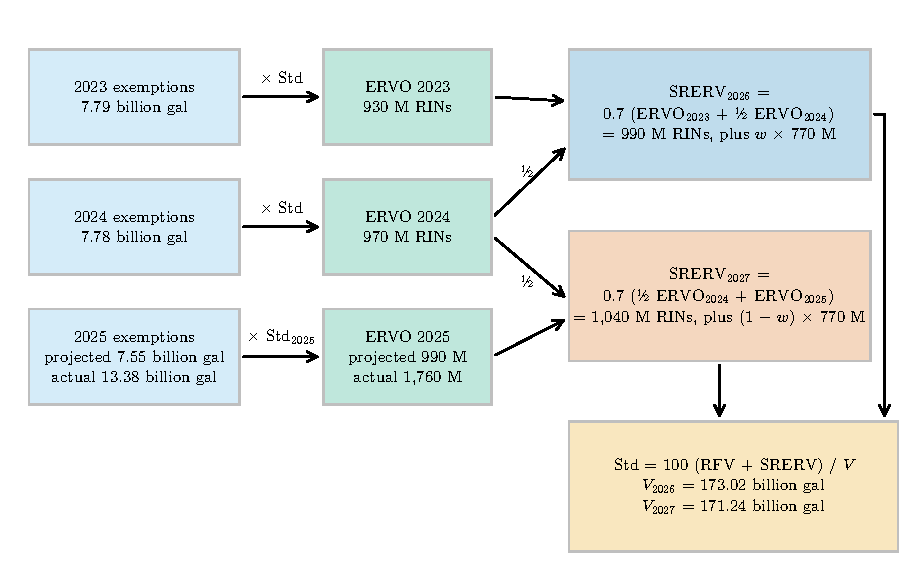
\includegraphics[width=\textwidth]{fig1_flow}
\caption{Flow of volumes from exemptions to standards. Exempted fuel volumes by year are multiplied by that year's standards to give exempted obligations (ERVO); 70~percent of the 2023--2025 obligations enters the 2026 and 2027 reallocation volumes (SRERV), and the additional 2025 obligation is assigned with share $w$ to 2026. Data basis: published values from 91~FR~16439--16440, 91~FR~65706 and docket document EPA-HQ-OAR-2024-0505-0789.}
\label{fig:flow}
\end{figure}

\begin{figure}[htbp]
\centering
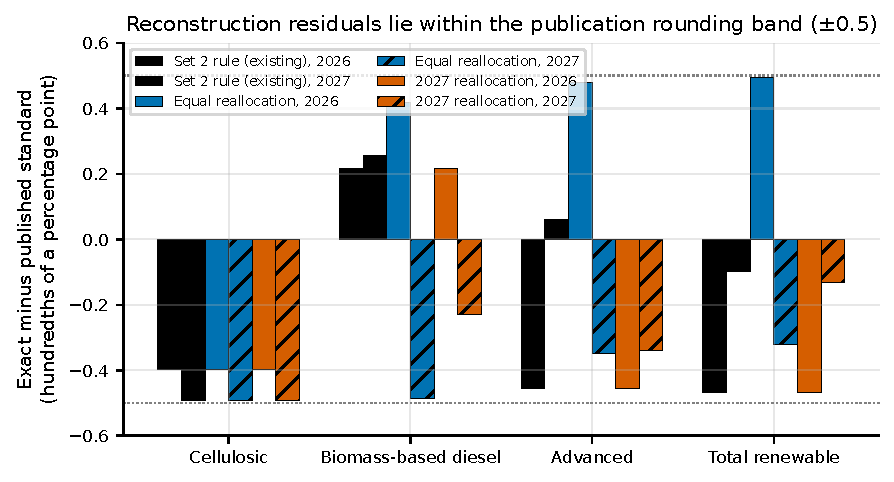
\includegraphics[width=\textwidth]{fig2_residuals}
\caption{Reproduction residuals: exact standard computed from the printed inputs minus the published two-decimal value, in hundredths of a percentage point, for every category and year of the Set~2 rule and the two alternatives (the eight no-reallocation standards are listed in Table~\ref{tab:reconstruction}). Data basis: computed from published inputs (observed).}
\label{fig:residuals}
\end{figure}

\begin{figure}[htbp]
\centering
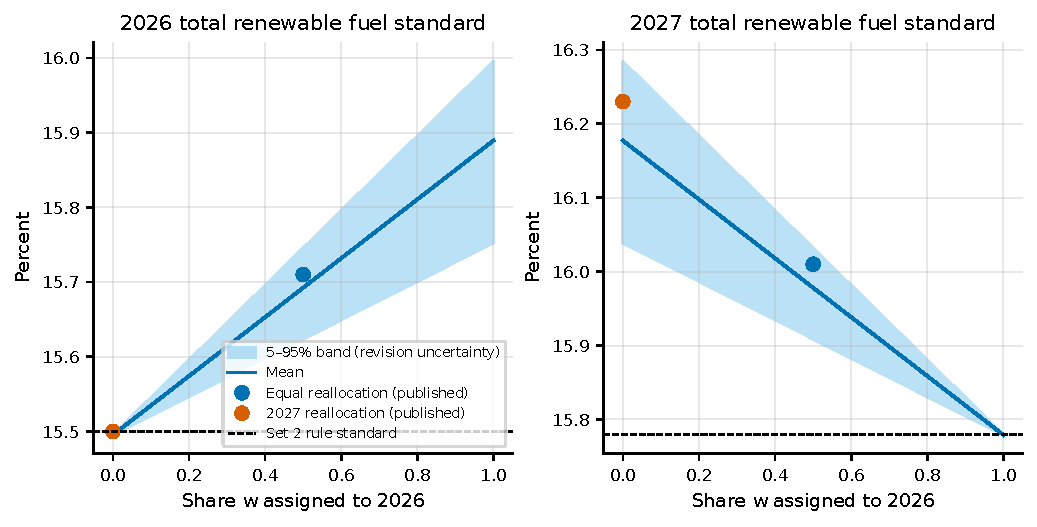
\includegraphics[width=\textwidth]{fig3_bands}
\caption{Total renewable fuel standard for 2026 and 2027 as a function of the share $w$ of the additional 2025 obligation assigned to 2026, with the 5--95~percent band from the empirical revision distribution (reported versus petition-based exempted obligations, \valnRevisionPairs{} years). Points are the published values of the two alternatives. Data basis: Monte Carlo on the empirical revision distribution (modelled); published values (observed).}
\label{fig:bands}
\end{figure}

\begin{figure}[htbp]
\centering
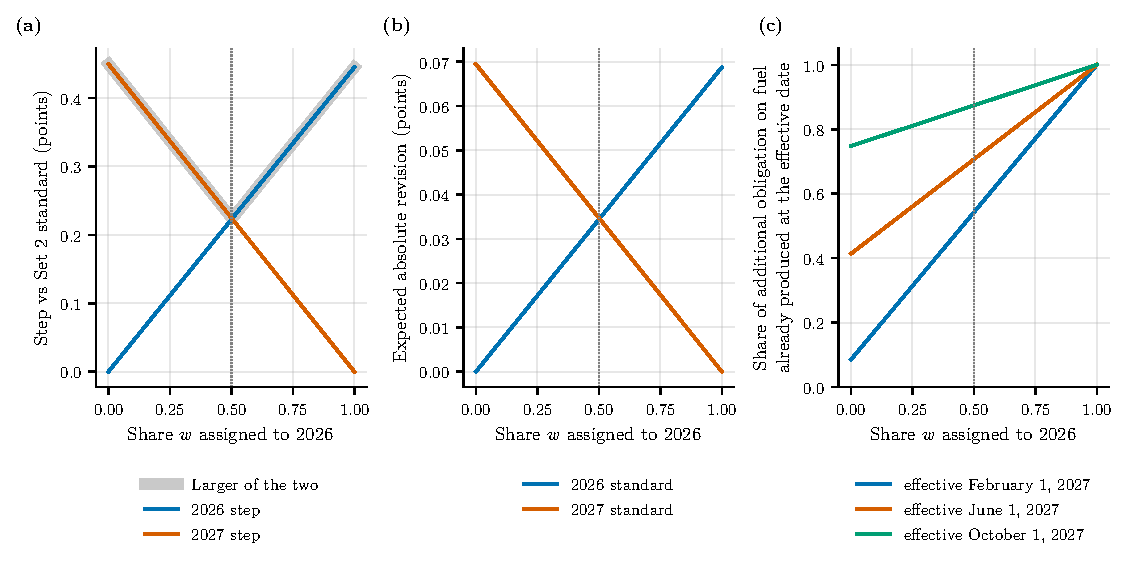
\includegraphics[width=\textwidth]{fig4_tradeoff}
\caption{Timing-rule trade-offs across $w$: step in each year's standard relative to the Set~2 rule (left), expected absolute revision of each standard if the exemption estimate is updated (centre, Monte Carlo), and share of the additional obligation imposed for an elapsed compliance period under three hypothetical final-rule effective dates (right). Data basis: deterministic and modelled; effective dates are hypothetical scenarios, not EPA projections.}
\label{fig:tradeoff}
\end{figure}

\begin{figure}[htbp]
\centering
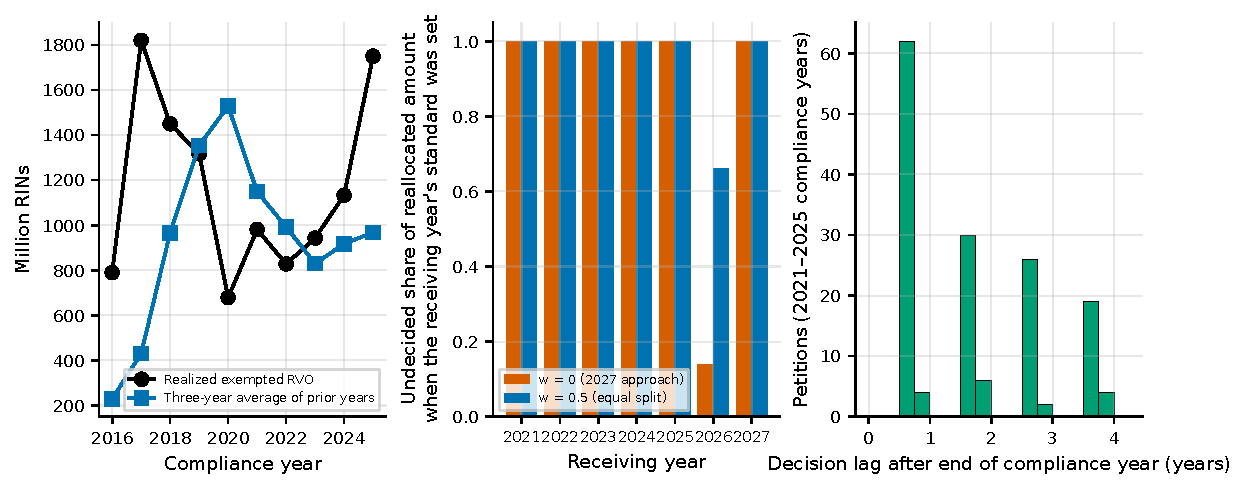
\includegraphics[width=\textwidth]{fig5_backtest}
\caption{Historical backtest. Left: realized exempted obligation by compliance year (EPA dashboard) and the three-year average of prior years. Centre: share of the amount a fixed timing rule would reallocate to each receiving year that was still undecided when that year's standard was set, for $w = 0$ and $w = 1/2$. Right: distribution of decision lags after the end of the compliance year for petitions for 2021--2025. Data basis: observed EPA record.}
\label{fig:backtest}
\end{figure}

\begin{figure}[htbp]
\centering
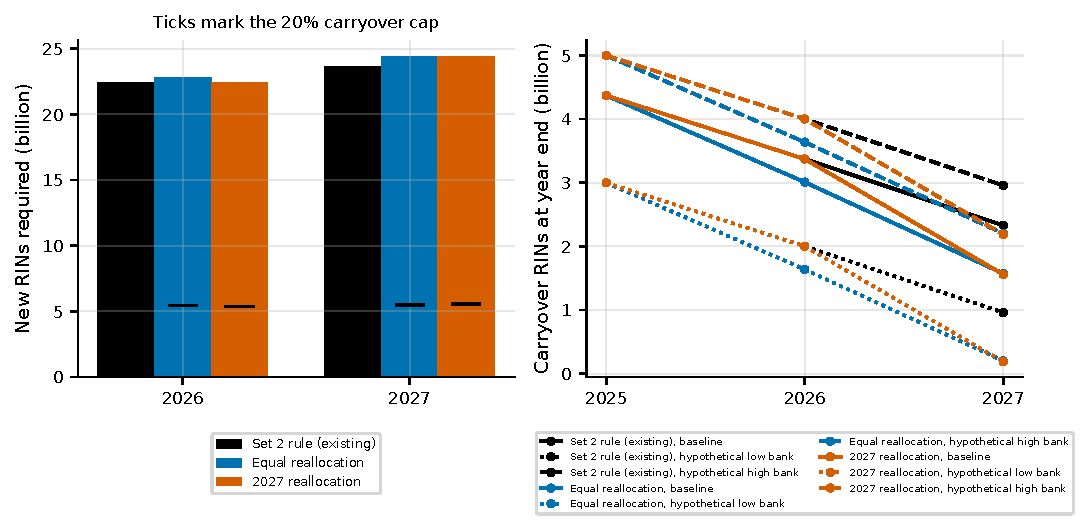
\includegraphics[width=\textwidth]{fig6_carryover}
\caption{Carryover accounting. Left: new RINs required in each year under each alternative with the baseline bank; ticks mark the 20~percent cap on prior-year RINs. Right: bank available at year end under the baseline and two hypothetical bank sizes. Data basis: accounting under stated assumptions (generation equal to the volume requirement); bank scenarios other than the baseline are hypothetical.}
\label{fig:carryover}
\end{figure}

\bibliographystyle{elsarticle-harv}
\bibliography{references}
\end{document}
